\documentclass{beamer}
\mode<presentation>
{
  \usetheme{Warsaw}
  \setbeamercovered{transparent}  
}
\usepackage[spanish]{babel}
\usepackage[utf8x]{inputenc}
\usepackage{default}
\title[Trabajo especial de la Licenciatura en Cs. de la Computaci\'on]
{Dise\~no de vacunas atenuadas con menor probabilidad de sufrir reversi\'on a
la virulencia}
\author[S.Videla, L.Alonso i Alemany, D.Rabinovich, D.Gutson]{S.Videla\inst{1}
\and L.Alonso i Alemany\inst{1} \and D.Rabinovich\inst{2,3} \and
D.Gutson\inst{3}}
\institute{
  \inst{1}Facultad de Matem\'atica, Astronom\'ia y F\'isica - Universidad
Nacional de C\'ordoba.
  \and
  \inst{2}Centro Nacional de Referencia para el SIDA. Facultad de Medicina -
Universidad Nacional de Buenos Aires.
  \and
  \inst{3}Fundaci\'on para el Desarrollo de la Programaci\'on en \'Acidos
Nucleicos.
}

\date[RCASAV 2010] % (optional, should be abbreviation of conference name)
{XXX Reuni\'on Cient\'ifica Anual de la Sociedad Argentina de Virolog\'ia, 2010}

\AtBeginSubsection[]
{
  \begin{frame}<beamer>{Contenidos}
    \tableofcontents[currentsection, currentsubsection]
  \end{frame}
}

\begin{document}
\begin{frame}
  \titlepage
\end{frame}

\section{Motivaci\'on}
\subsection{Vacunas atenuadas}
\begin{frame}
 \begin{itemize}
  \item Peligro de reversi\'on a la virulencia.
  \item Caso testigo: Vacuna Sabin contra la poliomielitis (OPV). \\
        $\Rightarrow$ Es conocido el rol del IRES y su estructura secundaria de
RNA en la atenuaci\'on.\\
        $\Rightarrow$ Queremos realizar un an\'alisis sistem\'atico de las
posibles variantes al IRES de los virus atenuados Sabin que conserven la
estructura secundaria de RNA.
 \end{itemize}
\end{frame}

\subsection{Objetivo}
\begin{frame}
Desarrollar un software que sirva como soporte para el dise\~no de vacunas
atenuadas m\'as seguras:
\begin{itemize}
 \item \textbf{Entrada:} Genoma del virus atenuado, genomas de los pat\'ogenos
o revertantes y un conjunto de restricciones (propiedades de inter\'es para la
atenuaci\'on de virus).
 \item \textbf{Objetivo:} Satisfaciendo las restricciones impuestas, maximizar
la distancia entre el genoma del virus atenuado y los genomas pat\'ogenos o
revertantes.
 \item \textbf{Salida:} Una o varias secuencias, candidatas a ``mejorar'' el
virus atenuado.
\end{itemize}
\end{frame}

\subsection{Antecedentes}
\begin{frame}
Algunos antecedentes en el dise\~no racional de vacunas atenuadas:
 \begin{itemize}
  \item Fidelidad en la replicaci\'on modificando la RNA polimerasa.
``\textit{Engineering attenuated virus vaccines by controlling replication
fidelity}''. Vignuzzi et al. 
  \item (De)-Optimizaci\'on de codones y pares de codones.
``\textit{Virus Attenuation by Genome-Scale Changes in Codon Pair Bias}''.
Coleman et al.
  \item Otras aproximaciones. ``\textit{Rationalizing the development of live
attenuated virus vaccines}''. Lauring et al.
 \end{itemize}
\end{frame}

\section{Propuesta}
\subsection{Formalizaci\'on del problema}
\begin{frame}
Sea $N$ la longitud de la secuencia de RNA del virus atenuado, y para $k
\in \mathbb{N}$ sea $\mathcal{S}_{k}$ el conjunto de secuencias de RNA de
longitud $k$. Entonces definimos:

\begin{itemize} 
 \item \textbf{Espacio de soluciones:} $\mathcal{S}_{N}$

 \item \textbf{Componentes variables de una soluci\'on:} $s_{1},s_{2}, \dots,
s_{n}$ tal que $s_{i} \in \mathcal{S}_{N_{i}}$ con $1 \le i \le n$ y $0 < N_{i}
\le N$.

 \item \textbf{Restricciones sobre las componentes:} Conservaci\'on de la
estructura secundaria o de la secuencia aminoac\'idica con respecto al virus
atenuado.

 \item \textbf{Funci\'on ``objetivo'' o de evaluaci\'on:} $f: \mathcal{S}_{N}
\rightarrow \mathbb{R}$ tal que $f(s)$ calcula la bondad de cada soluci\'on, en
nuestro caso, como la distancia en n\'umero de mutaciones necesarias para
llegar de $s$ a alguna secuencia pat\'ogena o revertante.
\end{itemize}
\end{frame}

\subsection{Optimizaci\'on combinatoria}
\begin{frame}
El problema de optimizaci\'on consiste en, iterativamente modificar el genoma
del virus atenuado asignado valores a las componentes $s_{1},s_{2}, \dots,
s_{n}$ asegurando que:
  \begin{itemize}
   \item los valores asignados satisfacen las restricciones impuestas sobre cada
componente.
   \item las secuencias que resultan de asignar valores a cada componente,
tiendan a maximizar la funci\'on $f$.
  \end{itemize}
 \begin{figure}
  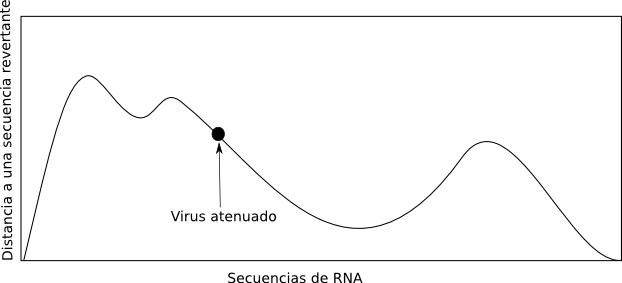
\includegraphics[scale=.5]{hillclimbing.png}
 \end{figure}
\end{frame}


\section{Aportes y trabajo futuro}
\subsection{Aportes}
\begin{frame}
 \begin{itemize}
  \item An\'alisis y formalizaci\'on del problema.
  \item Implementaci\'on del software como una prueba de concepto.
  \item Aplicable a cualquier virus (+)ssRNA.
 \end{itemize}
\end{frame}

\subsection{Trabajo futuro}
\begin{frame}
Queda pendiente tener en cuenta:
  \begin{itemize}
   \item Rango de temperaturas.
   \item Recombinantes con virus hom\'ologos.
   \item Otros tipos de virus RNA.
   \item Ensayos con datos reales.
  \end{itemize}
\end{frame}

\end{document}
